\documentclass[sigplan,10pt]{acmart}

\usepackage[normalem]{ulem} % \sout{} for strikethrough text
\usepackage{tikz}
\usetikzlibrary{arrows.meta,snakes}

\setcopyright{rightsretained}
\copyrightyear{2020}
\acmYear{2020}
\acmDOI{}
\acmConference[]{}{}{}
\acmBooktitle{}
\acmPrice{}
\acmISBN{}

\hyphenation{da-ta-cen-ter da-ta-cen-ters time-stamp time-stamps time-stamped hard-links}

\begin{document}
\title{Moving Elements in List CRDTs}

\author{Martin Kleppmann}
\email{mk428@cl.cam.ac.uk}
\orcid{0000-0001-7252-6958}
\affiliation{%
  \institution{University of Cambridge}
  \streetaddress{15 JJ Thomson Avenue}
  \city{Cambridge}
  \state{}
  \postcode{CB3 0FD}
  \country{United Kingdom}
}

\begin{abstract}
Conflict-free Replicated Data Types (CRDTs) for lists allow multiple users to concurrently insert and delete elements in a shared list object.
However, existing algorithms behave poorly when users concurrently move list elements to a new position (i.e.\ reorder the list elements).
We demonstrate the need for such a move operation, and describe an algorithm that extends a list CRDT with an explicit move operation.
Our algorithm can be used in conjunction with any existing list CRDT algorithm.
In addition to moving a single list element, we also discuss the open problem of moving ranges of elements.
\end{abstract}

\begin{CCSXML}
<ccs2012>
    <concept>
        <concept_id>10003752.10003809.10010172</concept_id>
        <concept_desc>Theory of computation~Distributed algorithms</concept_desc>
        <concept_significance>500</concept_significance>
    </concept>
    <concept>
        <concept_id>10011007.10010940.10010992.10010993.10010996</concept_id>
        <concept_desc>Software and its engineering~Consistency</concept_desc>
        <concept_significance>500</concept_significance>
    </concept>
    <concept>
        <concept_id>10003120.10003130.10003131.10003570</concept_id>
        <concept_desc>Human-centered computing~Computer supported cooperative work</concept_desc>
        <concept_significance>300</concept_significance>
    </concept>
    <concept>
        <concept_id>10002951.10003227.10003233</concept_id>
        <concept_desc>Information systems~Collaborative and social computing systems and tools</concept_desc>
        <concept_significance>300</concept_significance>
    </concept>
    <concept>
        <concept_id>10010520.10010521.10010537.10010540</concept_id>
        <concept_desc>Computer systems organization~Peer-to-peer architectures</concept_desc>
        <concept_significance>300</concept_significance>
    </concept>
</ccs2012>
\end{CCSXML}

\begin{CCSXML}
<ccs2012>
 </ccs2012>
\end{CCSXML}

\ccsdesc[500]{Theory of computation~Distributed algorithms}
\ccsdesc[500]{Software and its engineering~Consistency}
\ccsdesc[300]{Human-centered computing~Computer supported cooperative work}
\ccsdesc[300]{Information systems~Collaborative and social computing systems and tools}
\ccsdesc[300]{Computer systems organization~Peer-to-peer architectures}

\keywords{conflict-free replicated data types, distributed consistency, collaborative editing, optimistic replication}

\settopmatter{printfolios=true} % Recommended EuroSys formatting
\maketitle

\section{Introduction}

Conflict-free Replicated Data Types (CRDTs) allow multiple replicas to concurrently modify some shared data object, while ensuring that all replicas eventually converge towards the same, consistent state~\cite{Shapiro:2011un}.
CRDT algorithms have been developed for various different datatypes, and one of the most important datatypes is the \emph{list} (also called \emph{sequence} or \emph{array} datatype).
A list is a collection of elements in a total order, which is chosen by the user.

Replicated lists can be used to implement a variety of important applications, such as:
\begin{itemize}
    \item collaborative text editors (text is a list of characters);
    \item collaborative graphics applications (a list of graphical objects, where the order determines visibility: objects ``further down'' may be occluded or filtered by the objects ``higher up'', as illustrated in Figure~\ref{fig:smiley});
    \item to-do lists and task trackers (a list of tasks, where the order may reflect the relative priority of tasks as chosen by the user).
\end{itemize}

\begin{figure*}
  \centering
  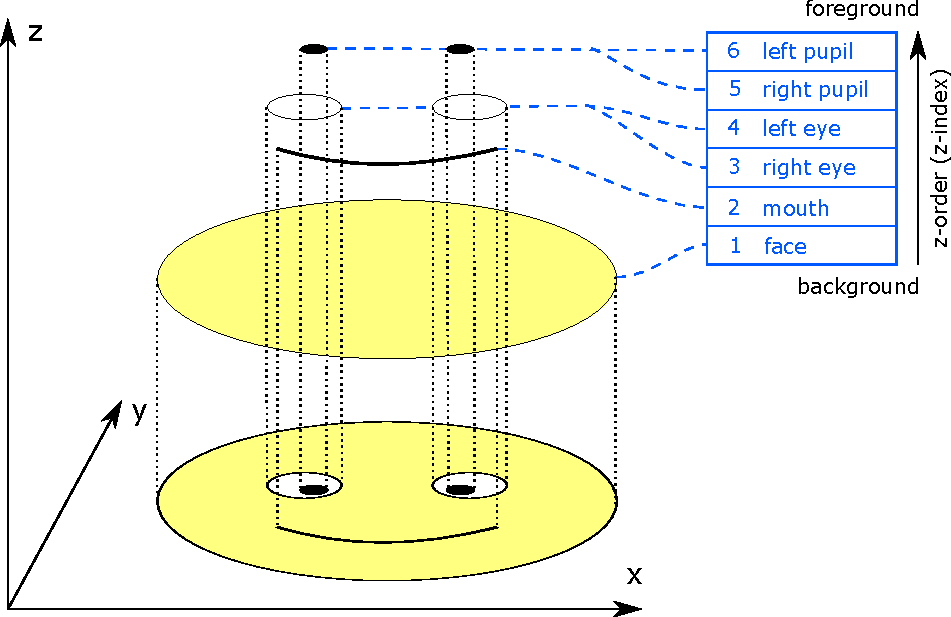
\includegraphics{smiley.pdf}
  \caption{Graphics software often places objects in a list that determines the z-index; objects higher in the list occlude lower ones. %
    Here, the eyeballs and mouth are placed above the yellow face, and the pupils in turn are placed above the eyeballs.}
  \label{fig:smiley}
\end{figure*}

Many list CRDTs have been developed, such as WOOT~\cite{Oster:2006wj}, Treedoc~\cite{Preguica:2009fz}, RGA~\cite{Roh:2011dw}, Causal Trees/Timestamped Insertion Trees~\cite{Grishchenko:2014eh,Attiya:2016kh}, Logoot \cite{Weiss:2009ht,Weiss:2010hx}, and LSEQ \cite{Nedelec:2013ky,Nedelec:2016eo}.
Moreover, most of the field of Operational Transformation algorithms is dedicated to algorithms for collaboratively editable text, i.e.\ lists~\cite{Ellis:1989ue,Nichols:1995fd,Ressel:1996wx,Sun:1998vf,Oster:2006tr}.

All of the aforementioned algorithms allow replicas to \emph{insert} or \emph{delete} elements anywhere in the list.
However, none of them have explicit support for \emph{moving} elements from one position to another position in the list (\emph{reordering}).
This is a surprising omission because moving is a commonly required operation: in many to-do list applications, a user can drag and drop list elements to reorder them, and graphics software allows users to reorder the object list with commands such as ``bring to front'' (which moves an object to the top of the list, so that it occludes other objects) and ``send to back'' (which moves an object to the bottom, so that it is occluded by other objects).

In this paper we introduce an algorithm that allows an existing list CRDT to be extended with a move operation.
The algorithm is generic in the sense that it can be implemented on top of any of the aforementioned list CRDTs.

\section{Semantics of Concurrent Moves}\label{sec:semantics}

The simplest way of moving a list element is to delete it from its existing position, and to re-insert it at the new position.
However, if two replicas concurrently move the same element, the result is that the element is duplicated: the two deletions of the same element behave the same as one deletion, and the two insertions independently re-insert the element twice.

\definecolor{insertcolor}{rgb}{0, 0.5, 0}
\definecolor{deletecolor}{rgb}{1, 0, 0}
\definecolor{movecolor}{rgb}{0.5, 0, 1}
\definecolor{networkcolor}{rgb}{0, 0.5, 1}

\begin{figure*}
    \centering
    \vspace{3em}
    \begin{tikzpicture}[auto,scale=1.0]
        \tikzstyle{item}=[rectangle,draw,inner ysep=4pt,text height=9pt,text depth=2pt,minimum width=2.2cm]
        \tikzstyle{network}=[thick,dashed,networkcolor,-{Stealth[length=3mm]}]
        \path [draw,dotted] (0,2) -- (17.5,2);
        \node at (1, 4) {Replica $A$:};
        \node at (1, 0) {Replica $B$:};
        \matrix [row sep={19pt,between origins},nodes=item] at (4, 4) {
            \node [minimum width=0.5cm] {1.}; & \node (top1) {buy milk}; \\
            \node [minimum width=0.5cm] {2.}; & \node {water plants}; \\
            \node [minimum width=0.5cm,fill=movecolor!10] {3.}; & \node [fill=movecolor!10] (joe1) {phone joe}; \\
        };
        \matrix [row sep={19pt,between origins},nodes=item] at (4, 0) {
            \node [minimum width=0.5cm] {1.}; & \node (top2) {buy milk}; \\
            \node [minimum width=0.5cm] {2.}; & \node {water plants}; \\
            \node [minimum width=0.5cm,fill=movecolor!10] {3.}; & \node [fill=movecolor!10] (joe2) {phone joe}; \\
        };
        \draw [->,movecolor,thick] (joe1.east) to [in=0, out=0] node [right,near end] {move} (top1.north east);
        \draw [->,movecolor,thick] (joe2.east) to [in=0, out=0] node [right,near end] {move} (top2.north east);
        \draw [->,thick] (6, 0) -- (8.5, 0);
        \draw [->,thick] (6, 4) -- (8.5, 4);
        \matrix [row sep={19pt,between origins},nodes=item] at (10, 4) {
            \node [minimum width=0.5cm,fill=movecolor!10] {1.}; & \node [fill=movecolor!10] {phone joe}; \\
            \node [minimum width=0.5cm] {2.}; & \node {buy milk}; \\
            \node [minimum width=0.5cm] {3.}; & \node {water plants}; \\
        };
        \matrix [row sep={19pt,between origins},nodes=item] at (10, 0) {
            \node [minimum width=0.5cm,fill=movecolor!10] {1.}; & \node [fill=movecolor!10] {phone joe}; \\
            \node [minimum width=0.5cm] {2.}; & \node {buy milk}; \\
            \node [minimum width=0.5cm] {3.}; & \node {water plants}; \\
        };
        \draw [->,thick] (11.5, 0) -- (14.5, 0);
        \draw [->,thick] (11.5, 4) -- (14.5, 4);
        \draw [network] (12.5, 0) to [out=90,in=270] (13.1, 4);
        \draw [network] (12.5, 4) to [out=270,in=90] (13.1, 0);
        \node [rotate=90,networkcolor,font=\footnotesize] at (13.5, 2) {network communication};
        \matrix [row sep={19pt,between origins},nodes=item] at (16, 4) {
            \node [minimum width=0.5cm,fill=movecolor!10] {1.}; & \node [fill=movecolor!10] {phone joe}; \\
            \node [minimum width=0.5cm,fill=movecolor!10] {2.}; & \node [fill=movecolor!10] {phone joe}; \\
            \node [minimum width=0.5cm] {3.}; & \node {buy milk}; \\
            \node [minimum width=0.5cm] {4.}; & \node {water plants}; \\
        };
        \matrix [row sep={19pt,between origins},nodes=item] at (16, 0) {
            \node [minimum width=0.5cm,fill=movecolor!10] {1.}; & \node [fill=movecolor!10] {phone joe}; \\
            \node [minimum width=0.5cm,fill=movecolor!10] {2.}; & \node [fill=movecolor!10] {phone joe}; \\
            \node [minimum width=0.5cm] {3.}; & \node {buy milk}; \\
            \node [minimum width=0.5cm] {4.}; & \node {water plants}; \\
        };
    \end{tikzpicture}
    \caption{If moving is implemented by deleting and re-inserting, concurrent moves of the same element result in the anomaly shown here: the moved element is duplicated.}
    \label{fig:duplication}
\end{figure*}

\begin{figure*}
    \centering
    \vspace{3em}
    \begin{tikzpicture}[auto,scale=1.0]
        \tikzstyle{item}=[rectangle,draw,inner ysep=4pt,text height=9pt,text depth=2pt,minimum width=2.2cm]
        \tikzstyle{network}=[thick,dashed,networkcolor,-{Stealth[length=3mm]}]
        \path [draw,dotted] (0,1.5) -- (17.5,1.5);
        \node at (1, 3) {Replica $A$:};
        \node at (1, 0) {Replica $B$:};
        \matrix [row sep={19pt,between origins},nodes=item] at (4, 3) {
            \node [minimum width=0.5cm] {1.}; & \node (top1) {buy milk}; \\
            \node [minimum width=0.5cm] {2.}; & \node {water plants}; \\
            \node [minimum width=0.5cm,fill=movecolor!10] {3.}; & \node [fill=movecolor!10] (joe1) {phone joe}; \\
        };
        \matrix [row sep={19pt,between origins},nodes=item] at (4, 0) {
            \node [minimum width=0.5cm] {1.}; & \node (top2) {buy milk}; \\
            \node [minimum width=0.5cm] {2.}; & \node {water plants}; \\
            \node [minimum width=0.5cm,fill=movecolor!10] {3.}; & \node [fill=movecolor!10] (joe2) {phone joe}; \\
        };
        \draw [->,movecolor,thick] (joe1.east) to [in=0, out=0] node [right,near end] {move} (top1.north east);
        \draw [->,movecolor,thick] (joe2.east) to [in=0, out=0] node [right,at end,inner xsep=8pt] {move} (top2.south east);
        \draw [->,thick] (6, 0) -- (8.5, 0);
        \draw [->,thick] (6, 3) -- (8.5, 3);
        \matrix [row sep={19pt,between origins},nodes=item] at (10, 3) {
            \node [minimum width=0.5cm,fill=movecolor!10] {1.}; & \node [fill=movecolor!10] {phone joe}; \\
            \node [minimum width=0.5cm] {2.}; & \node {buy milk}; \\
            \node [minimum width=0.5cm] {3.}; & \node {water plants}; \\
        };
        \matrix [row sep={19pt,between origins},nodes=item] at (10, 0) {
            \node [minimum width=0.5cm] {1.}; & \node {buy milk}; \\
            \node [minimum width=0.5cm,fill=movecolor!10] {2.}; & \node [fill=movecolor!10] {phone joe}; \\
            \node [minimum width=0.5cm] {3.}; & \node {water plants}; \\
        };
        \draw [->,thick] (11.5, 0) -- (14.5, 0);
        \draw [->,thick] (11.5, 3) -- (14.5, 3);
        \draw [network] (12.5, 0) to [out=90,in=270] (13.1, 3);
        \draw [network] (12.5, 3) to [out=270,in=90] (13.1, 0);
        \node [rotate=90,networkcolor,font=\footnotesize] at (13.5, 1.5) {network communication};
        \matrix [row sep={19pt,between origins},nodes=item] at (16, 3) {
            \node [minimum width=0.5cm,fill=movecolor!10] {1.}; & \node [fill=movecolor!10] {phone joe}; \\
            \node [minimum width=0.5cm] {2.}; & \node {buy milk}; \\
            \node [minimum width=0.5cm] {3.}; & \node {water plants}; \\
        };
        \matrix [row sep={19pt,between origins},nodes=item] at (16, 0) {
            \node [minimum width=0.5cm,fill=movecolor!10] {1.}; & \node [fill=movecolor!10] {phone joe}; \\
            \node [minimum width=0.5cm] {2.}; & \node {buy milk}; \\
            \node [minimum width=0.5cm] {3.}; & \node {water plants}; \\
        };
    \end{tikzpicture}
    \caption{When the same element is concurrently moved to different positions on different replicas, one of those positions should become the ``winning'' position as the replicas converge. In this example, replica $A$'s move operation wins.}
    \label{fig:concurrent}
\end{figure*}

We argue that such duplication in the face of concurrency is undesirable, as it is generally not the behaviour expected by users.
For example, say a user has replicas of their to-do list on their laptop and their smartphone.
They move items on their laptop to match new priorities, and also move some items on their phone while the phone is offline, as illustrated in Figure~\ref{fig:duplication}.
Later, when the phone is online again and synchronises with the laptop, any items that were moved on both devices will be duplicated.

This behaviour is especially confusing if the same item was moved to the same position (e.g.\ to the top of the list) on both devices, in which case the duplicated items are likely to be adjacent in the final list, as in Figure~\ref{fig:duplication} (depending on any other insertions that might have taken place).
However, even if the concurrent move operations had different destination positions, duplicating the moved element at both destinations is unlikely to be desirable behaviour in most applications.

Rather, we argue that the best semantics in this situation is for the system to pick one of the destination positions as the ``winner''; as the replicas communicate, they all converge towards a list in which the moved element is located only at the winning position, and nowhere else.
This approach is illustrated in Figure~\ref{fig:concurrent}.
Any deterministic method of picking the winner is suitable (e.g.\ based on a priority given to each replica, or based on the timestamp of the operations).

\begin{figure*}
    \begin{tikzpicture}
        \tikzstyle{state}=[matrix,anchor=west,column sep={18pt,between origins},row sep={18pt,between origins}]
        \tikzstyle{char}=[draw,anchor=base,minimum width=18pt,text height=8pt,text depth=3pt,minimum height=18pt]
        \tikzstyle{mov}=[fill=movecolor!10]
        \tikzstyle{ins}=[fill=insertcolor!10]
        \tikzstyle{del}=[fill=deletecolor!10]
        \tikzstyle{network}=[thick,dashed,networkcolor,-{Stealth[length=3mm]}]
        \path [draw,dotted] (0,1.5) -- (17.5,1.5);
        \node at (0, 4) [anchor=west] {Replica $A$:};
        \node at (0, 1) [anchor=west] {Replica $B$:};
        \node (before1) at (0,3) [state] {
            \node [char] {$\bullet$}; &
            \node [char] {}; &
            \node [char] {\texttt{B}}; &
            \node [char] {\texttt{a}}; &
            \node [char] {\texttt{c}}; &
            \node [char] {\texttt{o}}; &
            \node [char] {\texttt{n}}; &
            \node [char] {\verb|\n|}; &
            \node {}; &
            \node {}; &
            \node {}; &
            \node {}; \\
            \node [char] {$\bullet$}; &
            \node [char] {}; &
            \node [char,ins] (ins-begin) {\color{insertcolor}{\texttt{S}}}; &
            \node [char,ins] {\color{insertcolor}{\texttt{o}}}; &
            \node [char,ins] {\color{insertcolor}{\texttt{y}}}; &
            \node [char,ins] {}; &
            \node [char,ins] (ins-end) {\color{insertcolor}{\texttt{m}}}; &
            \node [char,del] (del) {\color{deletecolor}{\renewcommand{\ULthickness}{1pt}\sout{~\texttt{M}~}}}; &
            \node [char] {\texttt{i}}; &
            \node [char] {\texttt{l}}; &
            \node [char] {\texttt{k}}; &
            \node [char] {\verb|\n|}; &
            \node {}; \\
        };
        \draw [snake=brace,raise snake=3pt,gap around snake=1pt,insertcolor,thick]
            (ins-end.south east) -- node [midway,below,inner ysep=8pt] {insert} (ins-begin.south west);
        \draw [snake=brace,raise snake=3pt,gap around snake=1pt,deletecolor,thick]
            (del.south east) -- node [midway,below,inner ysep=8pt] {delete} (del.south west);
        \node (before2) at (0,0) [state] {
            \node [char] {$\bullet$}; &
            \node [char] {}; &
            \node [char] {\texttt{B}}; &
            \node [char] {\texttt{a}}; &
            \node [char] {\texttt{c}}; &
            \node [char] {\texttt{o}}; &
            \node [char] {\texttt{n}}; &
            \node [char] (dest) {\verb|\n|}; \\
            \node [char,mov] {$\bullet$}; &
            \node [char,mov] {}; &
            \node [char,mov] {\texttt{M}}; &
            \node [char,mov] {\texttt{i}}; &
            \node [char,mov] {\texttt{l}}; &
            \node [char,mov] {\texttt{k}}; &
            \node [char,mov] (src) {\verb|\n|}; &
            \node {}; \\
        };
        \draw [->,movecolor,thick] (src.east) .. controls +(0:2cm) and +(0:1cm) .. node [right,near end,inner xsep=7pt] {move} (dest.north east);
        \draw [->,thick] (6.2, 0) -- (10.0, 0);
        \draw [->,thick] (8.0, 3) -- (10.0, 3);
        \draw [network] (8.5, 0) to [out=90,in=270] (9.1, 3);
        \draw [network] (8.5, 3) to [out=270,in=90] (9.1, 0);
        \node [rotate=90,networkcolor,font=\footnotesize] at (9.5, 1.5) {network communication};
        \node (after1) at (10,3) [state] {
            \node [char,mov] {$\bullet$}; &
            \node [char,mov] {}; &
            \node [char,mov] {\texttt{M}}; &
            \node [char,mov] {\texttt{i}}; &
            \node [char,mov] {\texttt{l}}; &
            \node [char,mov] {\texttt{k}}; &
            \node [char,mov] {\verb|\n|}; &
            \node {}; \\
            \node [char] {$\bullet$}; &
            \node [char] {}; &
            \node [char] {\texttt{B}}; &
            \node [char] {\texttt{a}}; &
            \node [char] {\texttt{c}}; &
            \node [char] {\texttt{o}}; &
            \node [char] {\texttt{n}}; &
            \node [char] {\verb|\n|}; \\
            \node [char,ins] {\color{insertcolor}{\texttt{S}}}; &
            \node [char,ins] {\color{insertcolor}{\texttt{o}}}; &
            \node [char,ins] {\color{insertcolor}{\texttt{y}}}; &
            \node [char,ins] {}; &
            \node [char,ins] {\color{insertcolor}{\texttt{m}}}; &
            \node {}; &
            \node {}; &
            \node {}; \\
        };
        \node (after2) at (10,0) [state] {
            \node [char,mov] {$\bullet$}; &
            \node [char,mov] {}; &
            \node [char,mov] {\texttt{M}}; &
            \node [char,mov] {\texttt{i}}; &
            \node [char,mov] {\texttt{l}}; &
            \node [char,mov] {\texttt{k}}; &
            \node [char,mov] {\verb|\n|}; &
            \node {}; \\
            \node [char] {$\bullet$}; &
            \node [char] {}; &
            \node [char] {\texttt{B}}; &
            \node [char] {\texttt{a}}; &
            \node [char] {\texttt{c}}; &
            \node [char] {\texttt{o}}; &
            \node [char] {\texttt{n}}; &
            \node [char] {\verb|\n|}; \\
            \node [char,ins] {\color{insertcolor}{\texttt{S}}}; &
            \node [char,ins] {\color{insertcolor}{\texttt{o}}}; &
            \node [char,ins] {\color{insertcolor}{\texttt{y}}}; &
            \node [char,ins] {}; &
            \node [char,ins] {\color{insertcolor}{\texttt{m}}}; &
            \node {}; &
            \node {}; &
            \node {}; \\
        };
    \end{tikzpicture}
    \caption{Replica $B$ moves a range of characters (here, ``$\bullet$ Milk''), while concurrently replica $A$ makes an edit inside the same range. If the move is performed character-by-character, $A$'s edit remains at the old position, while its surrounding context has moved to a new position, leading to an anomalous outcome.}
    \label{fig:range-bad}
\end{figure*}

\section{A Generic Moving Algorithm}\label{sec:algorithm}

Intuitively, if we want to pick one winner from among several concurrent moves for the same element, we can use a long-established CRDT: a last-writer wins (LWW) register~\cite{Shapiro:2011wy,Johnson:1975we}.
We need one such register for each list element, containing the position of that element.
Moving an element to a new location is then merely a matter of updating the value of that element's register.

In general, we could also use a multi-value (MV) register~\cite{Shapiro:2011wy}, which would allow an element to exist at multiple positions in the list simultaneously after having experienced conflicting moves.
This is not the same as the duplication described in Section~\ref{sec:semantics}, since the multiple positions still belong to the same element, and a subsequent move would collapse them back into a single position again.
The MV register option can be used if the LWW behaviour (discarding all but one of the concurrent moves of the same element) is unacceptable.

Regardless of whether a LWW or MV register is used, this approach requires a stable way of referencing some position in the list (i.e.\ the value held by the register).
An integer index is not suitable, because an insertion or deletion at any position would require changing all of the indices following that position.
Fortunately, all known list CRDTs already incorporate schemes for stable position identifiers.
The details vary: Treedoc uses a path through a binary tree~\cite{Preguica:2009fz}, Logoot uses a list of (integer, replicaID) pairs~\cite{Weiss:2009ht}, RGA uses a so-called s4vector~\cite{Roh:2011dw}, Causal Trees/Timestamped Insertion Trees use a timestamp~\cite{Grishchenko:2014eh,Attiya:2016kh}, and so on.
But all of these approaches have in common that they can uniquely refer to a particular position in a list, in a way that is not affected by operations on other list positions.

Assume now that $p_1, p_2, \dots$ are position identifiers according to one of the aforementioned schemes, and $v_1, v_2, \dots$ are the values of list elements (e.g.\ to-do list items).
We can now model the state of the list as a set of $(\mathit{value}, \mathit{register})$ pairs contained in an add-wins set CRDT:
\begin{align*}
\mathit{state} = \mathrm{AWSet}(\{ & (v_1, \mathrm{LWWRegister}(p_1)),\\
    & (v_2, \mathrm{LWWRegister}(p_2)), \;\dots\})
\end{align*}
In some schemes (such as Treedoc, Logoot and LSEQ), the position identifiers themselves encode their relative ordering~\cite{Interleaving}, and thus no further state is required.
In others (such as RGA and CT), the list CRDT requires an additional data structure that determines the order in which position identifiers appear in the list.

In order to obtain the elements in their list order we need to query the above set by the position identifiers stored within the registers.
We can do this efficiently by treating the set of pairs as a table in a relational database and using a database index on the position-register column.
The index lets us efficiently find all the list elements with a particular position ID (or range of position IDs).

Note that when the position of a list element is changed, the old position identifier no longer has any value associated with it, and thus it should be regarded as nonexistent (like a tombstone in some CRDTs).
It is also possible for multiple list elements to have the same position identifier, and thus for several list elements to appear at the same position.
This is similar to having a multi-value register of values at each list position.
(Note this situation is different from our earlier use of a MV register, which was about one element having multiple positions, not one position having multiple elements.)

We can avoid having multiple list elements with the same position identifier by always creating a fresh position identifier as the destination of a move operation.
All of the aforementioned list CRDTs have methods of creating new, globally unique position identifiers for any location within a list.

This algorithm is a CRDT because its state is a straightforward composition of existing CRDTs.

\begin{figure*}
    \begin{tikzpicture}
        \tikzstyle{state}=[matrix,anchor=west,column sep={18pt,between origins},row sep={18pt,between origins}]
        \tikzstyle{char}=[draw,anchor=base,minimum width=18pt,text height=8pt,text depth=3pt,minimum height=18pt]
        \tikzstyle{mov}=[fill=movecolor!10]
        \tikzstyle{ins}=[fill=insertcolor!10]
        \tikzstyle{del}=[fill=deletecolor!10]
        \tikzstyle{network}=[thick,dashed,networkcolor,-{Stealth[length=3mm]}]
        \path [draw,dotted] (0,1.5) -- (17.5,1.5);
        \node at (0, 4) [anchor=west] {Replica $A$:};
        \node at (0, 1) [anchor=west] {Replica $B$:};
        \node (before1) at (0,3) [state] {
            \node [char] {$\bullet$}; &
            \node [char] {}; &
            \node [char] {\texttt{B}}; &
            \node [char] {\texttt{a}}; &
            \node [char] {\texttt{c}}; &
            \node [char] {\texttt{o}}; &
            \node [char] {\texttt{n}}; &
            \node [char] {\verb|\n|}; &
            \node {}; &
            \node {}; &
            \node {}; &
            \node {}; \\
            \node [char] {$\bullet$}; &
            \node [char] {}; &
            \node [char,ins] (ins-begin) {\color{insertcolor}{\texttt{S}}}; &
            \node [char,ins] {\color{insertcolor}{\texttt{o}}}; &
            \node [char,ins] {\color{insertcolor}{\texttt{y}}}; &
            \node [char,ins] {}; &
            \node [char,ins] (ins-end) {\color{insertcolor}{\texttt{m}}}; &
            \node [char,del] {\color{deletecolor}{\renewcommand{\ULthickness}{1pt}\sout{~\texttt{M}~}}}; &
            \node [char] {\texttt{i}}; &
            \node [char] {\texttt{l}}; &
            \node [char] {\texttt{k}}; &
            \node [char] {\verb|\n|}; &
            \node {}; \\
        };
        \draw [snake=brace,raise snake=3pt,gap around snake=1pt,insertcolor,thick]
            (ins-end.south east) -- node [midway,below,inner ysep=8pt] {insert} (ins-begin.south west);
        \draw [snake=brace,raise snake=3pt,gap around snake=1pt,deletecolor,thick]
            (del.south east) -- node [midway,below,inner ysep=8pt] {delete} (del.south west);
        \node (before2) at (0,0) [state] {
            \node [char] {$\bullet$}; &
            \node [char] {}; &
            \node [char] {\texttt{B}}; &
            \node [char] {\texttt{a}}; &
            \node [char] {\texttt{c}}; &
            \node [char] {\texttt{o}}; &
            \node [char] {\texttt{n}}; &
            \node [char] (dest) {\verb|\n|}; \\
            \node [char,mov] {$\bullet$}; &
            \node [char,mov] {}; &
            \node [char,mov] {\texttt{M}}; &
            \node [char,mov] {\texttt{i}}; &
            \node [char,mov] {\texttt{l}}; &
            \node [char,mov] {\texttt{k}}; &
            \node [char,mov] (src) {\verb|\n|}; &
            \node {}; \\
        };
        \draw [->,movecolor,thick] (src.east) .. controls +(0:2cm) and +(0:1cm) .. node [right,near end,inner xsep=7pt] {move} (dest.north east);
        \draw [->,thick] (6.2, 0) -- (10.0, 0);
        \draw [->,thick] (8.0, 3) -- (10.0, 3);
        \draw [network] (8.5, 0) to [out=90,in=270] (9.1, 3);
        \draw [network] (8.5, 3) to [out=270,in=90] (9.1, 0);
        \node [rotate=90,networkcolor,font=\footnotesize] at (9.5, 1.5) {network communication};
        \node (after1) at (10,3) [state] {
            \node [char,mov] {$\bullet$}; &
            \node [char,mov] {}; &
            \node [char,ins] {\texttt{S}}; &
            \node [char,ins] {\texttt{o}}; &
            \node [char,ins] {\texttt{y}}; &
            \node [char,ins] {}; &
            \node [char,ins] {\texttt{m}}; &
            \node [char,mov] {\texttt{i}}; &
            \node [char,mov] {\texttt{l}}; &
            \node [char,mov] {\texttt{k}}; &
            \node [char,mov] {\verb|\n|}; &
            \node {}; \\
            \node [char] {$\bullet$}; &
            \node [char] {}; &
            \node [char] {\texttt{B}}; &
            \node [char] {\texttt{a}}; &
            \node [char] {\texttt{c}}; &
            \node [char] {\texttt{o}}; &
            \node [char] {\texttt{n}}; &
            \node [char] {\verb|\n|}; &
            \node {}; &
            \node {}; &
            \node {}; &
            \node {}; \\
        };
        \node (after2) at (10,0) [state] {
            \node [char,mov] {$\bullet$}; &
            \node [char,mov] {}; &
            \node [char,ins] {\texttt{S}}; &
            \node [char,ins] {\texttt{o}}; &
            \node [char,ins] {\texttt{y}}; &
            \node [char,ins] {}; &
            \node [char,ins] {\texttt{m}}; &
            \node [char,mov] {\texttt{i}}; &
            \node [char,mov] {\texttt{l}}; &
            \node [char,mov] {\texttt{k}}; &
            \node [char,mov] {\verb|\n|}; &
            \node {}; \\
            \node [char] {$\bullet$}; &
            \node [char] {}; &
            \node [char] {\texttt{B}}; &
            \node [char] {\texttt{a}}; &
            \node [char] {\texttt{c}}; &
            \node [char] {\texttt{o}}; &
            \node [char] {\texttt{n}}; &
            \node [char] {\verb|\n|}; &
            \node {}; &
            \node {}; &
            \node {}; &
            \node {}; \\
        };
    \end{tikzpicture}
    \caption{The desired outcome of the scenario in Figure~\ref{fig:range-bad}.}
    \label{fig:range-good}
\end{figure*}

\section{Moving Ranges of Elements}\label{sec:ranges}

The algorithm of Section~\ref{sec:algorithm} allows a single list element to be moved at a time.
In some applications, a further challenge arises: we may want to move not just one element, but move an entire consecutive range of elements in one operation.
For example, in a text document, a user may want to move a section of text (e.g.\ a paragraph, or the text of a bullet point) to a different position in the text~\cite{Lord:2019bo}.

We might try to move a range of elements by moving each element individually.
However, this approach has a problem, which is illustrated in Figure~\ref{fig:range-bad}.
In this example, replica $B$ wants to swap the order of two bullet points in the text of a shopping list by moving the character range ``$\bullet$ Milk'' (including the bullet point character $\bullet$), while concurrently replica $A$ changes the text ``Milk'' to ``Soy milk''.
While the move is successful, the character insertions and deletion of $A$'s edit remain attached to the old position of ``Milk'' (near the end of the document, after ``Bacon$\backslash$n'').
This is the case because CRDTs for lists and text perform insertions and deletions at particular position IDs, which remain unchanged even as elements are moved to new position IDs.

In contrast, the desired outcome of this scenario is shown in Figure~\ref{fig:range-good}: we want $A$'s edit to apply in the context in which it was originally made, even if that context has since moved to a new position in the document.
In order to enable this semantics, it is not sufficient to move each element individually: we need to capture the fact that a certain range of elements is moved, so that any concurrent edits that fall within that range can be redirected to the new position of that range.

At present, there is no known algorithm for performing such moves of ranges of elements.
Various tricky edge-cases would need to be handled by such an algorithm, such as concurrent moves of partially overlapping ranges, and moves whose destination position falls within another range that is itself being moved.
Part of the solution may be to give each list element a unique identity that is independent from its position in the document, so that the position of a list element can be changed without changing its identity; insertions and deletions can then reference the \emph{identities} of their context, rather than their position IDs.

We will briefly discuss one more approach for moving ranges, and explain why it is not sufficient.
In the example of Figures~\ref{fig:range-bad} and~\ref{fig:range-good}, if the application needs to support reordering of bullet points, we might try to simplify the problem by using a two-level hierarchy instead of a flat sequence of characters.
That is, we can create a top-level list object in which each list element contains the entire content of a single bullet point, and use a separate text CRDT object for the content of each bullet point.
In this design, moving bullet points requires only a single-element move operation.

However, this approach has a different problem: when the user presses the enter key in the middle of the text of a bullet point, the usual behaviour in most editors is to split it into two bullet points.
Conversely, hitting the delete key while the cursor is positioned at the end of a bullet point's text usually joins it with the following bullet point's text.
If each bullet point is represented as a separate text object, these splitting and joining operations require moving a range of characters from one text object to another.

Thus, representing each bullet point as a single list element for the sake of moving does not actually obviate the need for moving ranges of characters.
As before, implementing move as delete-and-reinsert has the effect of duplicating text if two users concurrently split or join the same bullet point.
Thus, it seems that support for moving ranges of characters is an important feature for collaborative document editors.

% There is also a more specific open problem: fixing a typo in the middle of a paragraph while concuurrently the entire paragraph is deleted.

% When moving a range, take the identity timestamp of all but the last element and move them to the new location.
% For the last element, leave the identity timestamp in place, but move the value to the new location.
% Insertions and deletions use the identity timestamp to locate their position.
% Thus, if they fall within the moved range, their identity timestamp will be located at the new location.

% The move operation itself also has a timestamp.
% When performing the move, for all elements but the last one in the range, we also pick up any intervening elements.
% (Can we say anything about the timestamps of those elements relative to the move operation's timestamp?)

% When moving two different ranges to the same destination position, need to ensure they end up in a deterministic order.
% Use positionID timestamps for this.

% When moving two partially overlapping ranges... how to ensure we don’t end up matching half the document?

% xdst ... lots of text ... xstart ... ystart ... xend ... yend ... ydst

% If x is moved to xdst first, then y second, the range of y would appear to include “lots of text”

% How to ensure the destination does not fall within the range being moved?


% bounds of range are given as positions (so that moving a range containing a bound does not move
% the bound somewhere else), but insertions/deletions reference element identity

% Inserted item may be relocated if its insertion position is within a range that was moved. This
% implies the insertion position cannot be given as a position ID in the operation, since a new
% position ID would have to be generated in the effector. However, if insertion contains only
% identity timestamp, as in RGA, then it’s fine?

% But then if a range’s bounds are specified as position IDs, and an insertion contains only an
% identity timestamp, where do the position IDs come from?

% Maybe an insert op should contain two timestamps — one for identity, one for position?


\section{Related work}

Our previous unpublished work \cite{ExtendedVersion} discusses a single-element move operation for lists in the context of a larger specification framework for CRDTs.
However, this work does not provide an efficient implementation of this operation.

Apart from this work, to our knowledge Ahmed-Nacer et al.~\cite{AhmedNacer:2013eq} provide the only published list CRDT that includes a single-element move operation.
However, it is designed to duplicate an element when moved concurrently~-- semantics we consider undesirable.
Moreover, we believe the algorithm to be more complicated than necessary.

All other list CRDTs~\cite{Oster:2006wj,Preguica:2009fz,Roh:2011dw,Grishchenko:2014eh,Attiya:2016kh,Weiss:2009ht,Weiss:2010hx,Nedelec:2013ky,Nedelec:2016eo} and Operational Transformation algorithms \cite{Ellis:1989ue,Nichols:1995fd,Ressel:1996wx,Sun:1998vf,Oster:2006tr} provide only insertion and deletion.

Lord~\cite{Lord:2019bo} discusses the problem of moving ranges of elements, but does not present a solution.

\section{Conclusions}

This short paper has made the case for list CRDTs to support an explicit move operation, allowing list elements to be reordered without duplicating them in the case of concurrent moves.
We have outlined an algorithm for single-element moves that can be retrofitted to any existing list CRDT that uses stable position IDs to refer to locations within the list (which is the case for all currently known list CRDTs).
We have also demonstrated the need for moving a contiguous range of list elements to a new position; finding an algorithm that adds this feature to a CRDTs is at present an open problem.
We hope that future research will succeed in developing an algorithm for moving ranges of elements.

\begin{acks}
Martin Kleppmann is supported by a Leverhulme Trust Early Career Fellowship and by the Isaac Newton Trust.
\end{acks}

\balance
\bibliographystyle{ACM-Reference-Format}
\bibliography{references}{}
\end{document}
